\section{Autopilot Design}
\subsection{}
The first order Nomoto model is a simple vessel model that we can use for this problem. The transfer function from rudder angle $\delta$ to heading rate $r = \dot \psi$ is given by equation (7.28) in \cite{Fossen2011} and is
\begin{equation}\begin{aligned}
\label{eq:nomoto_tf}
\frac{r}{\delta}(s) = \frac{K}{Ts + 1}
\end{aligned}\end{equation}
This corresponds to the time-domain representation
\begin{equation}\begin{aligned}
T \ddot \psi + \dot \psi = K \delta.
\end{aligned}\end{equation}

\subsection{}
In order to find the Nomoto parameters $T$ and $K$, we look at the step response of the system when excited by a reference $\delta_{\text{max}} = -25^{\circ}$, i.e. the maxiumum allowed rudder angle. Solving \eqref{eq:nomoto_tf} for the step response $r(t)$ we find
\begin{equation}\begin{aligned}
r(t) = \delta_{\text{max}} KT(1 - e^{-\frac{t}{T}}).
\end{aligned}\end{equation}
From classic control theory, we know that when $t = T$, $1 - e^{-\frac{t}{T}} = 1 - e^{-1} \approx 0.63$. In other words, the step response will hit $63\%$ of the final heading rate value $r_{\infty}$ at $t = T$. From \figref{fig:nomoto_reading} we see that this is at approximately $t = 140s$. Furthermore, as time goes to infinity, the exponential term goes to zero, and so $r$ approaches $\delta_{\text{max}} K T$. We read $r_\infty \approx 6.5 \cdot 10^{-3}$ from \figref{fig:nomoto_reading} and can then find $K$ as
\begin{equation}\begin{aligned}
K = \frac{r_{\infty}}{\delta_{\text{max}} T} \approx \frac{6.5 \cdot 10^{-3}}{25^{\circ} \cdot 140} \approx 1.06 \cdot 10^{-4}.
\end{aligned}\end{equation}
In total, we define the parameters
\begin{equation}\begin{aligned}
T = 140, \quad \text{and} \quad K = 1.06 \cdot 10^{-4}.
\end{aligned}\end{equation}

\begin{figure}[H]
\centering
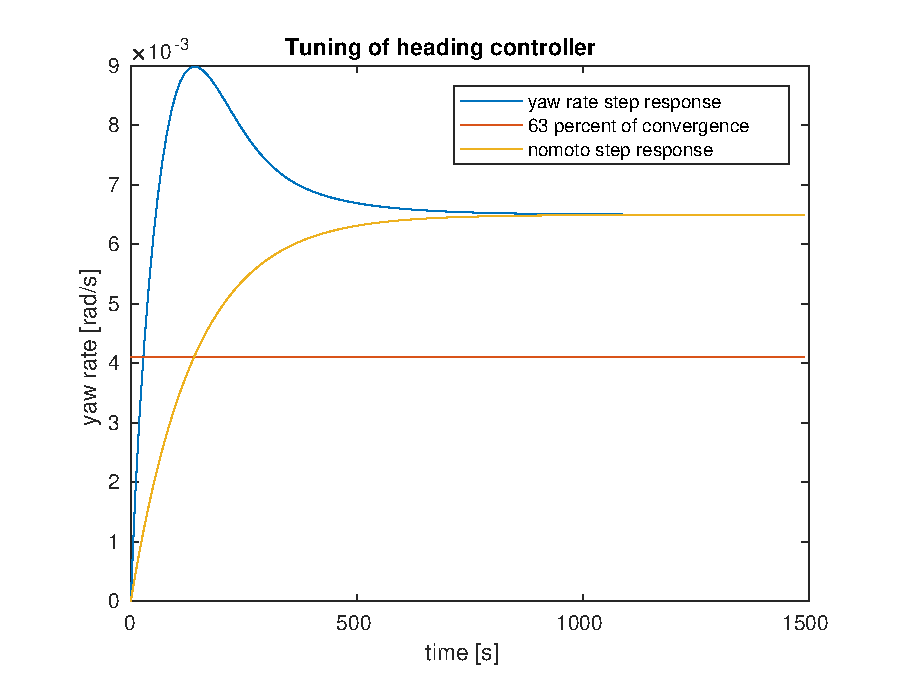
\includegraphics[width=0.7\textwidth]{nomoto-reading-improved}
\caption{Nomoto model parameter reading}
\label{fig:nomoto_reading}
\end{figure}


\subsection{}
We define a PD controller to control the heading $\psi$ from the rudder, i.e. we want the commanded rudder to be
\begin{equation}\begin{aligned}
\delta_c = -K_p (\psi_d - \psi) - K_d \dot \psi.
\end{aligned}\end{equation}
We wish to use the first order Nomoto model to find good values for $K_p$ and $K_d$. Using the model parameters, we define
\begin{equation}\begin{aligned}
T' = T \frac{U}{L_{pp}}, \quad K' = K \frac{L_{pp}}{U},
\end{aligned}\end{equation}
where $U = \sqrt{u^2 + v^2}$ is the ship velocity and $L_{pp}$ is the ship length. We also define
\begin{equation}\begin{aligned}
\omega_n = \sqrt{(\frac{u}{L_{pp}}) (\frac{1}{T})}, \quad \text{and} \quad \xi = 1.
\end{aligned}\end{equation}
With this, we choose the controller parameters
\begin{equation}\begin{aligned}
K_p = (\frac{L_{pp}}{U})^2 \frac{T'}{K'}, \quad \text{and} \quad
K_d = \frac{2 \xi \omega_n - 1}{K' \frac{U}{L_{pp}}}.
\end{aligned}\end{equation}
Note how the controller parameters depend on the current state of the system: they vary with the vessel velocity. Moreover, since we divide by the velocity $U$ in these expressions, the control law is clearly not defined for zero velocity. This is expected, since we obviously lose controllability for a velocity-driven heading control system when the velocity is zero.

In addition, since this control input will be input into a physical rudder, we have to saturate $\delta_c$ between the minimum and maximum rudder angles $-\delta_{\text{max}}$ and $\delta_{\text{max}}$. In addition, we could add rate limitation to the input, but we have not implemented this.

\subsection{}
We implement the controller as a simulink block and drive it with the reference
\begin{equation}\begin{aligned}
\psi_d(t) = 0.4 \sin (0.004t), \quad \text{and} \quad
r_d(t) = \dot \psi_d(t).
\end{aligned}\end{equation}
This, when simulated with current turned on, results in the heading shown in \figref{fig:heading1_4}. As we can see, we achieve acceptable tracking of the commanded heading. \figref{fig:rudder1_4} shows how the commanded rudder maxes out within the saturation limits. This is however not a problem for the heaidng controller.

\begin{figure}[ht]
	\centering
	\begin{subfigure}[b]{0.3\textwidth}
		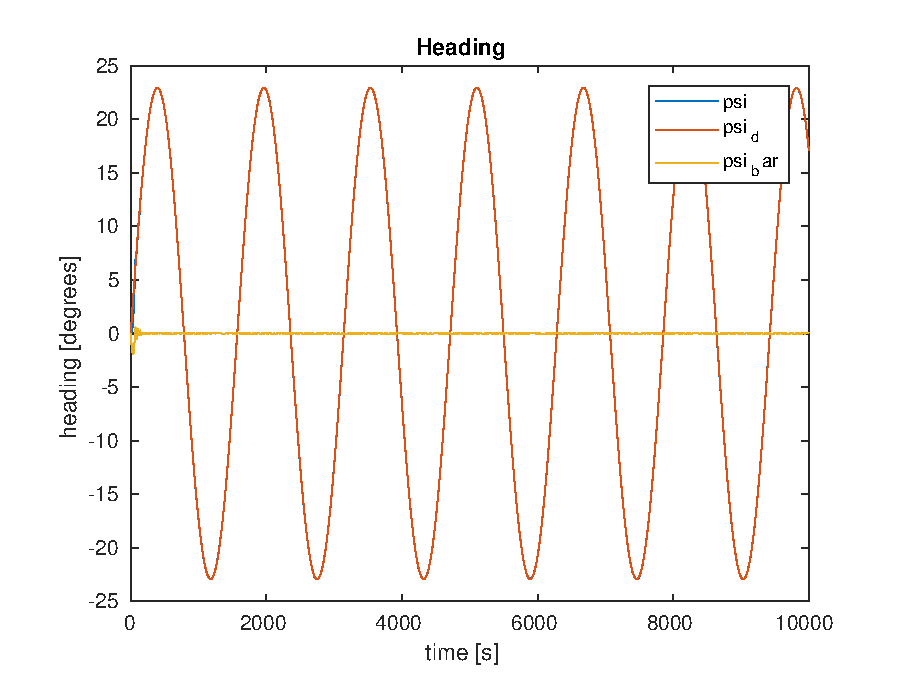
\includegraphics[width=\textwidth]{heading1_4}
		\caption{Heading}
		\label{fig:heading1_4}
	\end{subfigure}%
	~
	\begin{subfigure}[b]{0.3\textwidth}
		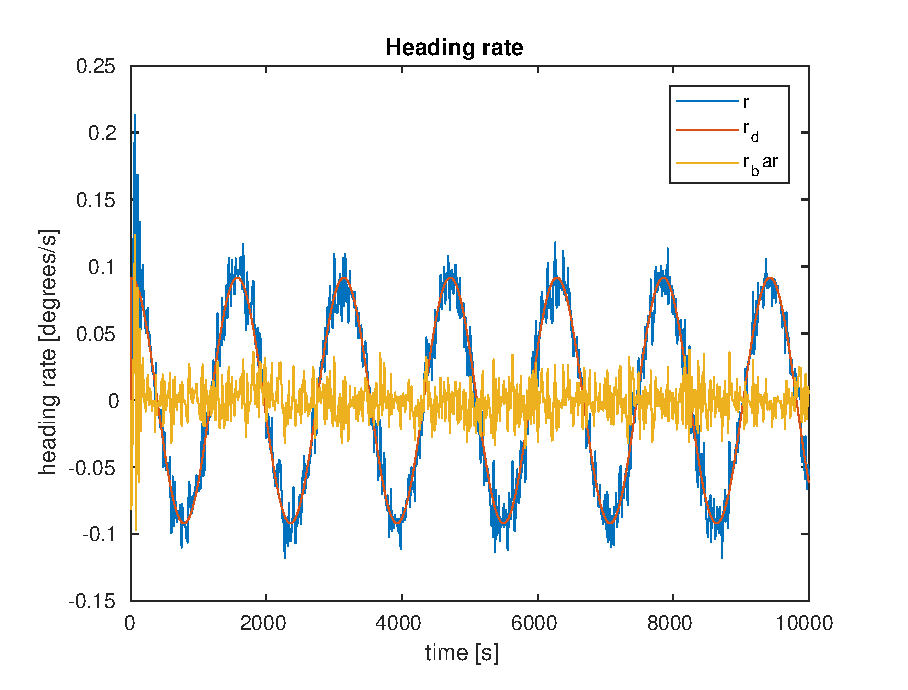
\includegraphics[width=\textwidth]{heading_rate1_4}
		\caption{Heading rate}
		\label{fig:heading_rate1_4}
	\end{subfigure}%
        ~
	\begin{subfigure}[b]{0.3\textwidth}
		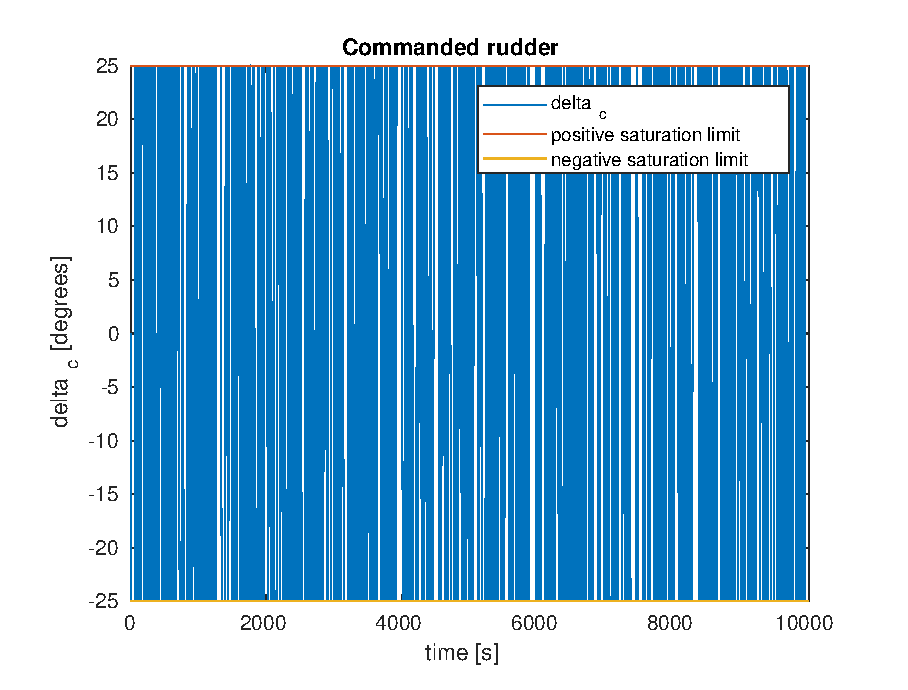
\includegraphics[width=\textwidth]{rudder1_4}
		\caption{Rudder with saturation}
		\label{fig:rudder1_4}
	\end{subfigure}
	\caption{Heading controller results}\label{fig:2}
\end{figure}

\subsection{}
To simplify further analysis, we hope to be able to fit a first order model to the surge dynamics. That is a model of the form
\begin{equation}\begin{aligned}
\frac{u}{n_c}(s) = \frac{K_u}{1 + T_u s},
\end{aligned}\end{equation}
where $u$ is surge speed and $n_c$ is the commanded shaft speed.


\subsection{}
We apply the same method for finding $T_u$ and $K_u$ as we did for finding the Nomoto model parameters, that is, we apply a step $n_{c,\text{step}}$ to the system and record the time constant as the time where the responds hits the $63 \%$ mark. We then find $K_u$ as $K_u = \frac{u_{\infty}}{n_{c,\text{step}}}$. For $n_{c,\text{step}} = 4$ we obtain
\begin{equation}\begin{aligned}
T_u = 790s, \quad \text{and} \quad K_u = 0.8157.
\end{aligned}\end{equation}
A comparison of the ship response and the model response given this step input is shown in \figref{fig:surge_boi}. As we can see, the non-linear overshoot of the ship is much less significant for the surge than for the heading, and so the deviation is less severe in this case.
\begin{figure}[H]
\centering
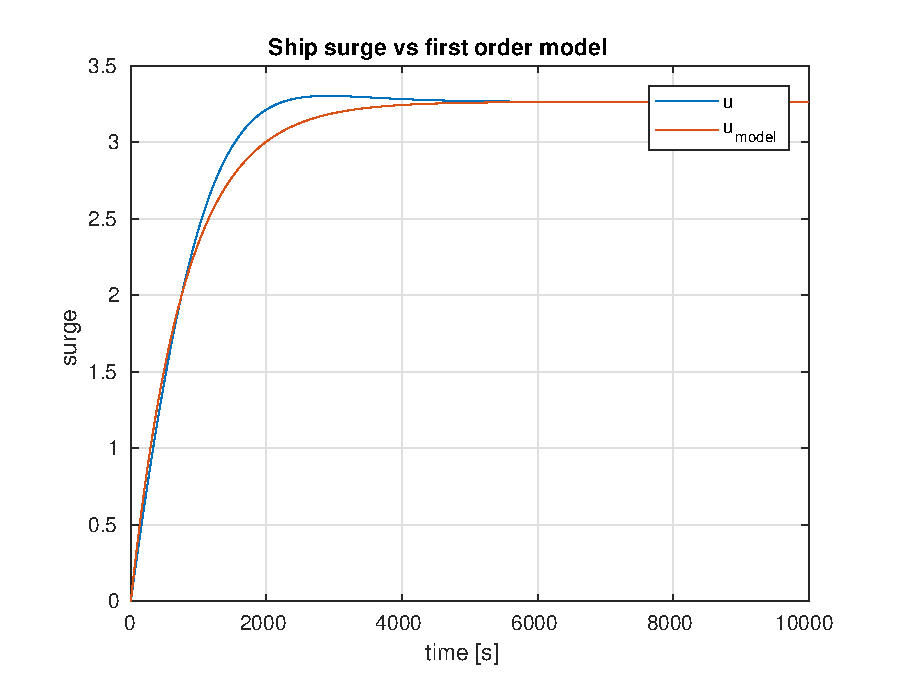
\includegraphics[width=0.7\textwidth]{surge_boi}
\caption{Ship surge dynamics vs first order model}
\label{fig:surge_boi}
\end{figure}

\subsection{}
To make a controller that can compensate for the current, we choose a PI controller, i.e. a controller of the form
\begin{equation}\begin{aligned}
n_c(t) = K_p \tilde u + K_i \int^{t}_{0} \tilde u,
\end{aligned}\end{equation}
where $\tilde u = u_d - u$.
For the controller parameters, we chose values
\begin{equation}\begin{aligned}
K_p = n_{c, \text{max}} = \frac{85 \cdot 2 \cdot \pi}{60}, \quad \text{and} \quad K_i = \frac{K_p}{T_u}.
\end{aligned}\end{equation}
The integral term is implemented by continuously summing the error term $\tilde u$ for each timestep, however since $n_c$ is saturated to be below $n_{c, \text{max}} = \frac{85 \cdot 2 \cdot \pi}{60}$, care must be taken to prevent integrator windup, i.e. prevent the integrator from accumulating a disproportionately large value while the controller is saturated. The simplest solution is to simply stop the summation when the controller is saturated, which is what we have implemented.

As for limitations, this controller, unlike the heading controller, does not lose controllability in any situation. Because of the integrator, it can follow constant references without producing static offset. In addition, the integrator will integrate slowly varying environmental effects such as current.


\subsection{}
We simulate the system with a step response from $u_d = 3$ to $u_d = 7$ at $t=1250s$. This results in the surge speed response shown in \figref{fig:heading1_7}. As we can see, the surge is affected by current, but the controller is able to compensate adequately. \figref{fig:rudder_shaft1_7} shows how $n_c$ does not go over the saturation limit. \figref{fig:surge_v_model1_7} shows the ship compared to the reference model, and clearly their responses are similar, but the first order model is a bit slower. We also note the small static offset. This could potentially be reduced by increasing the integral gain of the controller.

\begin{figure}[ht]
	\centering
	\begin{subfigure}[b]{0.45\textwidth}
		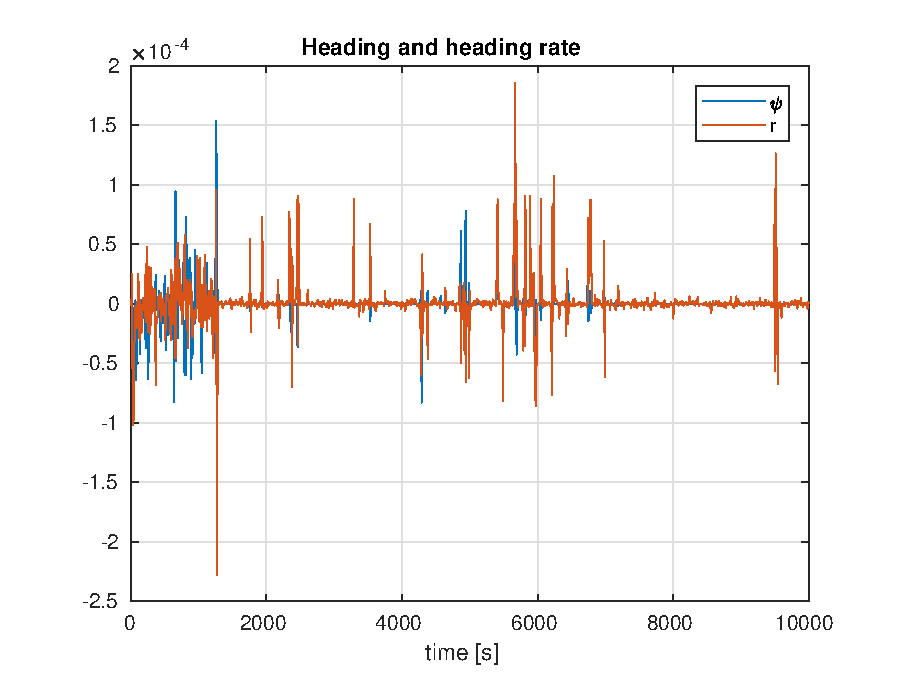
\includegraphics[width=\textwidth]{heading1_7}
		\caption{Heading}
		\label{fig:heading1_7}
	\end{subfigure}%
	~
	\begin{subfigure}[b]{0.45\textwidth}
		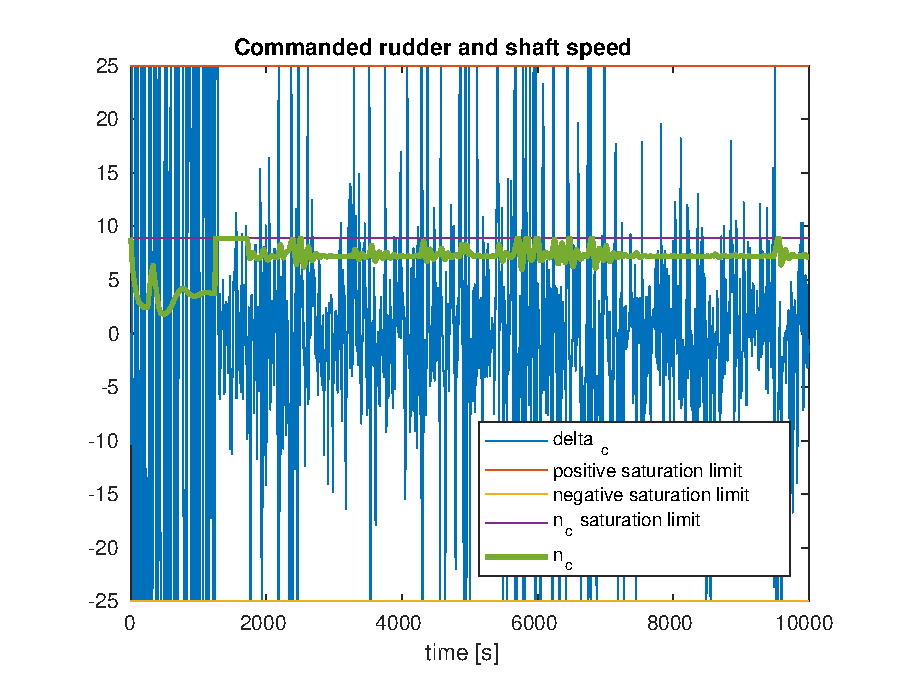
\includegraphics[width=\textwidth]{rudder_shaft1_7}
		\caption{Commanded rudder and shaft speed}
		\label{fig:rudder_shaft1_7}
	\end{subfigure}%

	\begin{subfigure}[b]{0.45\textwidth}
		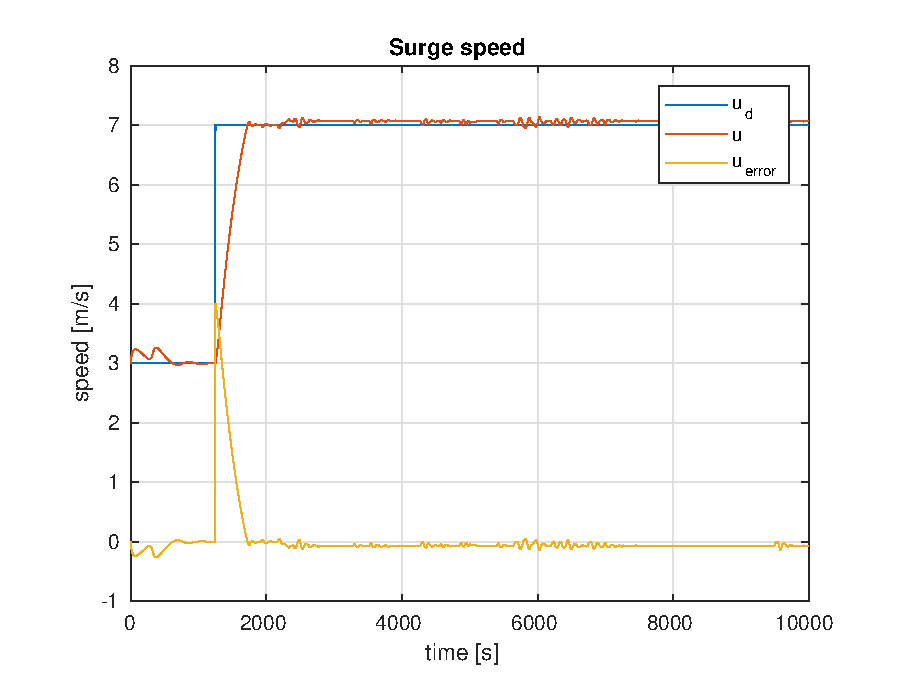
\includegraphics[width=\textwidth]{surge1_7}
		\caption{Surge speed}
		\label{fig:surge1_7}
	\end{subfigure}%
        ~
	\begin{subfigure}[b]{0.45\textwidth}
		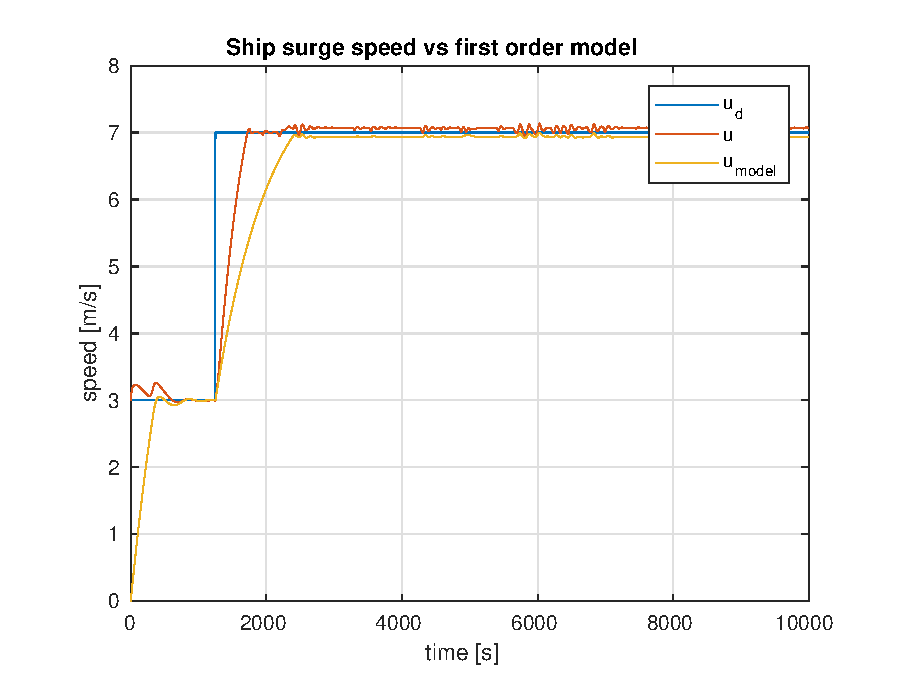
\includegraphics[width=\textwidth]{surge_v_model1_7}
		\caption{Ship vs model surge}
		\label{fig:surge_v_model1_7}
	\end{subfigure}
	\caption{Surge speed controller results}\label{fig:1_7}
\end{figure}
